\section{Implementation}

Our MLCache prototype was built on top of the Linux kernel version 4.14.0-rc7.
In this section, we provide a brief background to the page cache implementation
on Linux and describe how we modified it in order to add the learning model
described in Section~\ref{section:learning}.

\subsection{The Linux Page Cache}

Linux employs a modified version of the traditional LRU strategy called
\emph{two-list LRU}. As the name suggests, two LRU lists are maintained in this
approach: the \emph{active} and \emph{inactive} list. The active list contains
pages that have been accessed more than once in the past, whereas the inactive
list holds the set of pages that have been accessed only once. In other words,
the active list attempts to capture \emph{frequency} and the inactive list
captures \emph{recency}.

The following subsections introduce the main concepts that are relevant to our
work on MLCache. Figure~\ref{fig:lru} describes the two-list approach used in Linux.

\begin{figure}[h]
  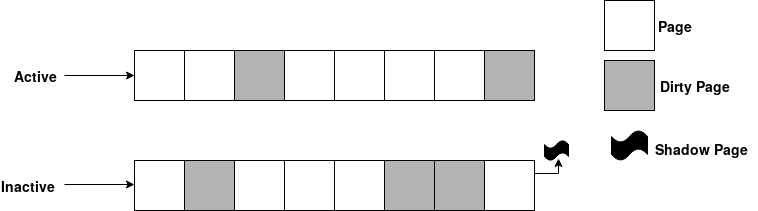
\includegraphics[scale=0.3]{img/LinuxLRU.png}
  \caption{The two-list LRU page cache on Linux. When a page is evicted (last
  page of the inactive list), it is replaced by a shadow page.}
  \label{fig:lru}
\end{figure}

\subsubsection{Dirty Pages}

As mentioned previously, the page cache holds blocks of data stored in the disk
device.  When user space applications perform write operations to certain
blocks of data, the corresponding pages are marked \emph{dirty}. Dirty pages
contain data that has not yet been flushed to the persistence device. In Linux,
dirty pages are not immediately flushed to the disk when the write operation
occurs; instead, the kernel periodically schedules a \emph{ writeback thread}
that scans the LRU lists and writes dirty pages to the disk.

\subsubsection{Cache Eviction}

When pages are read from or written to the disk, new entries are added to the
page cache.  As long as there is enough memory on the system, the number of
pages will keep growing, up to a certain threshold\footnote{Even a special
webpage was \cite{lamr} created in order to clarify this behavior, which
probably scares unfamiliar users.}. When the system is under memory pressure,
the kernel will create separate threads that will \emph{shrink} the LRU lists.
In particular, pages at the tail of the inactive LRU list are removed (pages
are always added to the head of an LRU list.) For this reason, Linux also
periodically ensures that the active and inactive lists are balanced: for
example, if too many pages are in the active list, the ones at the tail will be
demoted to the inactive list.

\subsubsection{Page Lookup}

Every page I/O operation on Linux goes through the page cache --- if the an
entry is found (\emph{cache hit}), an expensive call to the disk driver is
saved. Since these page lookups happen very often, they need to take a very
short time to produce a result. Linux 2.6 introduced a new page cache lookup
algorithm using \emph{radix trees} (as opposed to the old, global hash table in
previous kernels.) Each file contains its own radix tree of pages, and lookups
happen by providing only a file offset. Figure~\ref{fig:radix} illustrates the
radix tree approach, as defined in Linux 4.14.0-rc7.

\begin{figure}[h]
  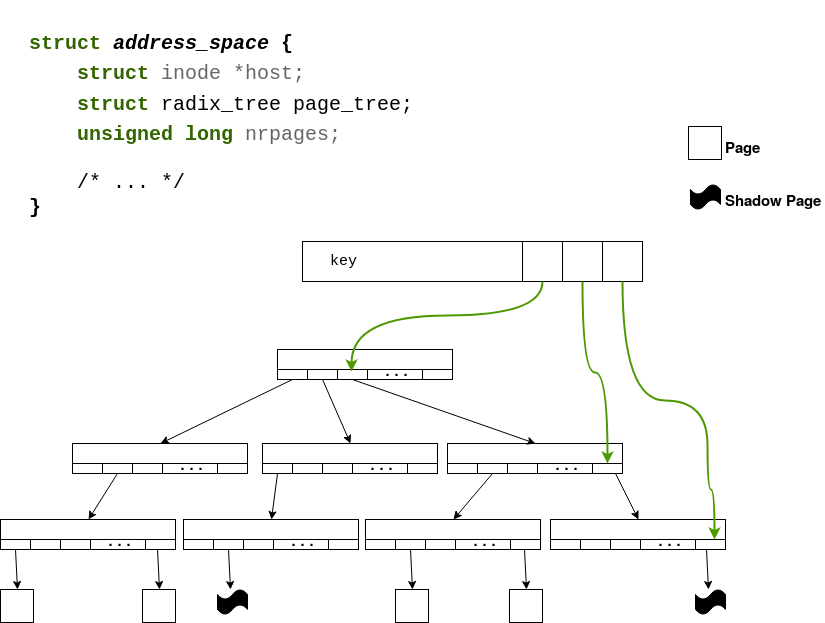
\includegraphics[scale=0.3]{img/LinuxRadixTree.png}
  \caption{The Linux page tree. Each file is represented by a (poorly named)
  \texttt{struct address\_space}, and contains a radix tree with pointers to
  locations where pages are kept in memory. When a page is evicted, a shadow
  page is placed in its previous spot. In the example lookup of this figure,
  \texttt{key} resolves to an entry with a shadow page. The corresponding page
  will likely be loaded directly into the \emph{active} LRU list.}
  \label{fig:radix}
\end{figure}

Another important aspect of the Linux implementation of radix trees is that nodes
can be marked with \emph{tags} --- the page cache uses this functionality to
indicate whether pages are dirty, unevictable, or a series of other attributes.
Nodes may also be marked \emph{exceptional}, a feature that is used to detect
shadow pages in the radix tree.

\subsubsection{Shadow Pages} \label{sss:shadow}

Another important optimization employed by the Linux page cache implementation
is the use of \emph{shadow pages}. Whenever a page is evicted, a special entry
--- called shadow page --- is created and replaces the spot previously occupied
by the recently evicted page in the radix tree. When a page lookup occurs and a
shadow page is found at the requested offset, the new page is added to the page
cache and inserted directly into the active LRU list. The use of shadow pages
is a cheap optimization (the shadow page is 8 bytes long, whereas a page is 4 KB
in x86) that can potentially avoid workflows that would cause thrashing.

\subsection{Page Scoring}

MLCache automatically calculates the score for each page based on the algorithm
described in Section~\ref{section:learning}. Specifically, for every page definition
(\texttt{struct page}), MLCache adds two new fields: the current page score, and
the number of times the page was previously evicted. In order for the algorithm
to work, the page scores need to remain accurate at all times.

Fortunately, Linux supports a \emph{tracepoint} API. More precisely, events can be
defined and, once included in a source file, be triggered with certain arguments.
MLCache introduces a new tracepoint, \texttt{mlcache\_event}, which is supposed
to be used whenever a page is requested. The event accepts a series of parameters
including a pointer to the \texttt{struct address\_space} involved, a pointer to the
page itself, the offset requested, and whether it was a hit or a miss. The newly
added event is triggered from within the \texttt{find\_get\_page} function in Linux.

\subsection{The \texttt{mlcache} Driver}

MLCache also introduces a new Linux driver, which coordinates its execution. The
driver's main tasks are:

\begin{description}
  \item[Update page scores] When this driver is loaded, it registers a function to be
    executed whenever the \texttt{mlcache\_event} tracepoint is triggered. This function
    rewards the page being requested and penalizes the other pages in the cache by
    traversing the associated radix tree.

  \item[Allow configuration by system operators] While
    MLCache can potentially improve the performance of a large class of applications,
    it is convenient to allow the system operator to selectively choose which applications
    should use MLCache's algorithms. That is done by writing to the \texttt{/proc/mlcache/}
    \texttt{filter}
    file that MLCache creates when it is loaded. Currently, MLCache is able to monitor either
    a list of processes or the process tree under a certain ID. For instance, the command:
\begin{verbatim}
    echo tree:$$ >/proc/mlcache/filter
\end{verbatim}
    causes MLCache to monitor every process
    under the running shell.

  \item[Read collected information] When monitoring a process, MLCache will create a file
    under the \texttt{/proc/mlcache} directory named after the identifier of the monitored process.
    By reading that file, system operators can analyze statistics about page cache hits/misses.
\end{description}

\subsection{Leveraging Shadow Pages}

As described in \ref{sss:shadow}, Linux uses shadow pages to optimize access to frequently accessed
pages even if they happen to be evicted due to high memory pressure. In our work, we extend the information
contained in the shadow page to include MLCache's scoring data. More specifically, whenever a page
is evicted from the page cache, we include both the current page score, as well as the number of times
the page was previously evicted in the created shadow page. Thus, when a page request finds a shadow
page, it can be brought back to the cache with the score it used to have before evicition. Figure~\ref{fig:shadow}
illustrates how the shadow page is structured when MLCache is enabled.

\begin{figure}[h]
  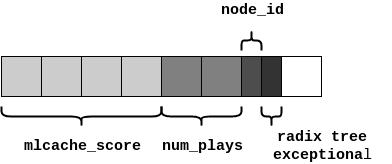
\includegraphics[scale=0.4]{img/ShadowPage.png}
  \caption{The Linux shadow page when MLCache is enabled. Each square
  represents one byte of information.  The shadow page is 8 bytes long and
  contains a series of data --- CPU node identifier, a radix tree entry indicating
  this is an exceptional node, among others. MLCache adds a 4 bytes long page
  score, as well as a 2 bytes long counter, indicating the number of times that
  page was previously evicted.}
  \label{fig:shadow}
\end{figure}

\subsection{Cache Eviction}

The final component of MLCache's implementation is the changed cache eviction policy. Cache eviction
on Linux happens when the amount of memory consumed by the page cache is above a certain threshold.
When pages need to be evicted, kernel threads will be awaken and both the active and inactive
LRU lists may be \emph{shrinked}. The shrinking process happens by evicting the last \texttt{n}
pages in an LRU list (where the value of \texttt{n} is determined at runtime depending on the
system's memory pressure.)

MLCache changes the LRU shrinking process by choosing the pages with the worst score. Unfortunately,
LRU lists are maintained as a linked list of pages, and choosing the pages to evict in LRU is a
constant time operation. Since MLCache needs to determine which pages have the worst score overall,
a linear scan over the LRU list is introduced in this step. Even though better data structures could
be leveraged in order to optimize the eviction process, we see positive results for some workloads
in our benchmarks, despite this unfavorable situation.
